\section{Distributed File Systems}

Big data can have different forms. You cn either have a huge amounts of large files or large amounts of huge files. I.e. Billions of TB files vs. Millions of PB files. For the first case, we use Key-Value Model and Object storage and for the second one we use File System and Block Storage.

\subsection{Main Requirements of a Distributed File System}

\paragraph{Fault tolerance and robustness} Local dist might fail, but in clusters with 100s to 10,000s of machines, the nodes will fail! Thus, storage technologies must be capable of: monitoring itself, detecting failures, automatically recovering and fault being, in the end and as a whole, fault tolerant.

\paragraph{File read and update model}
You can either have random access, meaning any part of the disk can be read and written at any time, and in any order. For distributed data storage, and for reading and writing large datasets, random access is not needed. We rather need to be able to efficiently scan a large file (in its entirety) - for data analysis, and be able to append efficiently new data at the end of an existing large file - particularly for logging sensors. We need to make sure that if one client is appending something to a file, another client cannot simultaneously add something to the file. This is called atomic.

\paragraph{Performance requirements}
Top priority: the bottleneck must be throughput. We do not want the bottleneck to be latency. Remember: the discrepancy between capacity and throughput can be resolved by parallelism and the discrepancy between throughput and latency can be resolved by batch processing.


\subsection{The Model behind HDFS}

\paragraph{File Hierarchy}
The HDFS cluster organizes its files as a hierarchy, called the file namespace. Files are thus organized in directories, similar to a local file system. (In a Key-Value Model we talk about objects, whereas in a File Hierarchy we talk about files.)

\paragraph{Blocks}
Unlike in S3, HDFS files are furthermore not stored as monolithic blackboxes, but HDFS exposes them as lists of blocks - also similar to a local file system. (Block Storage instead of Object Storage, where the whole data is saved as one big block.) The blocks are even exposed to the user. Files in an HDFS Cluster are stored as a list of blocks.

Why do we need blocks? For PB-sized files, we cannot fit the whole data on one machine (as of right now). Second, it is a level of abstraction simple enough that can be exposed on the logical level. Third, blocks can easily be spread at will across many machines.

\paragraph{The size of the blocks}
Typical sizes of blocks are 4 kB for a simple file system, 4 kB - 32 kB for a relational database and 64 MB - 128 MB for HDFS. Thsi is because of the prerequisits of HDFS: first, it is not optimized for random access, and second, blocks will be shipped over the network. 128 MB is a good sweetspot such that the blocks are large enough that the time not lost in latency, and at the same time small enough for a large file to be conveniently spread over many machines, allowing for parallel access, and also small enough for a block to be sent again without too much overhead in case of a network issue.


\subsection{Physical Architecture}
How is the cluster of machines connected? One way to connect machines is called peer-to-peer, decentralized network. In this network architecture, each machine talks to any other machine. By contrast, HDFS is implemented on a fully centralized architecture, in which one node is special and all others are interchangeable and connected to it. In HDFS we call the different nodes Namenode and Datanode.

If we want to store a file on HDFS we need to devide the data into 128 MB chunks called Block and distribute them among the datanodes. However, we also replicate them. Each block is stored three times. Each of these blocks is called a replica and they to not have a particular order. This enables to still be able to access the datablocks, eventhough a datanode might be down. Furthermore, you can also distribute the blocks among the globe, and a client can access the node closest to him or her in order to retrieve the data the fastest.

\subsubsection{The responsibilities of the NameNode}
The NameNode is responsible for the system-wide activity of the HDFS cluster. It stores in particular three things:
\begin{itemize}
    \item The File Namespace: The hierarchy of directory names and file names, as well as any access control (ACL) information similar to Unix-based systems.
    \item A mapping from each file to the list of its blocks. Each block in this list is represented with a 64-bit identifier; the content of the blocks is not on the NameNode.
    \item A mapping from each block represented with its 64-bit identifier, to the locations of its replicas, that is, the list of the DataNodes that store a copy of this block.
\end{itemize}
The NameNode updates this information whenever a client connects to it in order to update files and directories, as well as with the regular reports it receives from the DataNodes. Clients connect to the NameNode via the Client Protocol. Clients can perform metadata operations such as creating or deleting a directory, but also ask to delete a file, read a file or write a new file. In the latter case, the NameNode will send back to the client block identifiers (for reading them), or lists of DataNode locations (for reading and writing them).

\subsubsection{The responsibilities of the DataNode}
The DataNodes store the blocks themselves. These blocks are stored on their local disk.
DataNodes send regular heartbeats to the Namenode with a frequency (configurable) of a few seconds. DataNodes also send, every couple of hours, a full report including all the blocks that it contains.
If there is an issue with the local disk or the node, then the DataNode can report the block as corrupted to the NameNode, which will then ensure, asynchronously, its replication to somewhere else. "Asynchronously", as opposed to “synchronously,”, means that this is done in the background at some later time and the DataNode does not wait for this to happen.
NameNodes never connect to the DataNodes. They wait until the next heartbeat of the DataNode and answer to it with the request if there is one.

\begin{figure}[h]
    \centering
    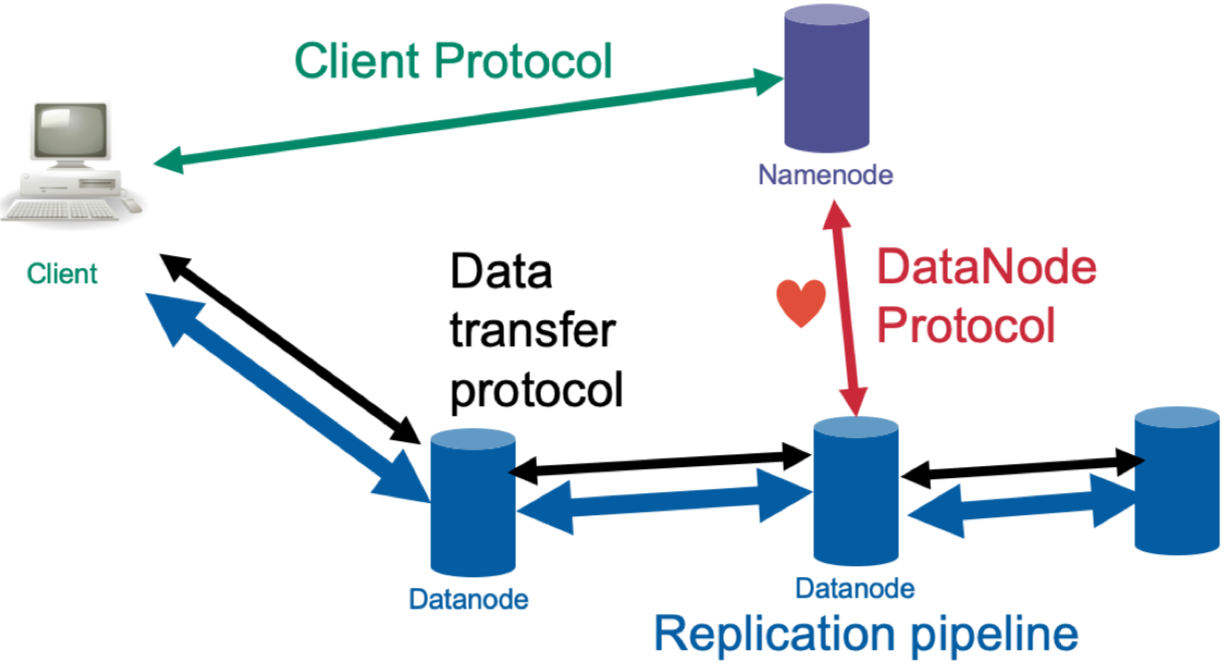
\includegraphics[width=0.7\textwidth]{Figures/ClientProtocol.png}
    \caption{Client Protocol}\label{fig:ClientProtocol}
\end{figure}

\paragraph{Client Protocol}
The NameNode is the first Node the Client will interact with.
A client can perform Metadata operations (create a directory, create a file, delete a file, etc.) and the NameNode will send back the DataNode location and Block IDs. This is all doable with a Java API.

\paragraph{DataNode Protocol}
The DataNode always initiates the connection! The DataNode sends information about the Registration, Heartbeat (every 3s), BlockReport (every 6h) and BlockReceived to the NameNode and the Name node returns Block operations.

\paragraph{Data Transfer Protocol (Streaming)}
The Client is only going to connect to the closest node, and when creating a file, the client does not need to connect to two other DataNodes to store the copy of the file, but the DataNodes will to that themselves.


\subsubsection{File System Functionality}

Metadata functionalities include \textit{Create directory, Delete directory, Write file, Append to file, Read file} and \textit{Delete file}.

\paragraph{Reading a File}
First, the client needs to connect to the NameNode to initiate the read and request info on the file. Then, the NameNode responds with the list of all blocks, as well as a list of DataNodes that contains a replica of each block. The DataNodes are furthermore sorted by increasing distance of the client (which is typically itself one of the nodes in the cluster, we will come back to this). The client then connects to the DataNodes in order to download a copy of the blocks. It starts with the first (closest) DataNode in the list provided by the NameNode for each blocks, and will go down the list if a DataNode cannot be reached or is not available. In the simple case that the client wants to stream its way through an HDFS file, bit by bit, it will download each block in turn. Note that with streaming, it is possible to process files larger than the working memory, because older blocks can be thrown away from the memory of the client once processed.

\paragraph{Write a file}
The client first conneects to the NameNode formulating its intent to create a new file. The NameNode will respond with the Block ID and a list of DataNodes to which the content of the first block should be sent. At that point the file is not yet guaranteed to be available for read for other clients, and it is locked in such a way that nobody else can write to it at the same time. The client then connects to the first DataNode and instructs it to organize a pipeline with the other DataNodes provided by the NameNode for this block. The client then starts sending through the content of that block, as we explained earlier. The content will be pipelined all the way to the other DataNodes. The client receives regular acknowledgements from the first DataN- ode that the bits have been received. When all bits have been acknowledged, the client connects to the NameNode in order to move over to the second block. Then, the same steps (2, 3, 4, 5) as before are repeated for each block. Once the last block has been written, the client informs the Na- meNode that the file is complete, and asks to release the lock. The NameNode then checks for minimal replication through the DataNode protocol and gives its final acknowledgement to the client. From now on, and separately (this is called “asynchronous”), the NameNode will continue to monitor the replicas and trigger copies from DataNode to DataNode whenever necessary, that is, when a block is underreplicated.

\subsection{Replication Strategy}
There is no order for the replicas and there usually are three replicas. How is it decided where the copies are stored? We need to consider reliability, Read/Write Bandwidth and Block distribution. One can define a distance between two nodes. The distance is defined as the "number of connecting lines between two nodes". If two nodes are in the same rack, the distance is equal to two (one from node A to the Rack, and one from the rack to node B). If two nodes are in diferent racks but still in the same cluster, then the distance is 4 (node A $\rightarrow$ Rack 1 $\rightarrow$ Cluster $\rightarrow$ Rack 2 $\rightarrow$ Node B). There are some rules where to store the replicas.
\begin{itemize}
    \item Replica 1: Same node as client (or random), rack A
    \item Replica 2: a node in a different rack B
    \item Replica 3: a node in same rack B
    \item Replica 4 and beyond: random, but if possible:
        \begin{itemize}
            \item at most one replica per node
            \item at most two replicas per rack
        \end{itemize}
\end{itemize}

\subsection{Fault Tolerance and Availability}
HDFS has a single point of failure: the NameNode. If the metadata stored on it is lost, then all the data on the cluster is lost, because it is not possible to reassemble the blocks into files any more. For this reason the metadata is backed up. More precisely, the file namespace containing the directory and file hierarchy as well as the mapping from files to block IDs is backed up to a so-called snapshot. Note that the mapping of block IDs to DataNodes does not require a backup, as it can be recovered from the periodic block reports (heartbeats). Since the HDFS system is constantly updated, it would not be viable to do a backup upon each update. It would also not be viable to do backups less often, as this could lead to data loss. Thus, what is done is that updates to the file system arriving after the snapshot has been made are instead stored in a journal, called edit log, that lists the updates sorted by time of arrival. The snapshot and edit log are stored either locally or on a network- attached drive (not HDFS itself). For more resilience, they can also be copied over to more backup locations. If the NameNode crashes, it can be restarted, the snapshot can be loaded back into memory to get the file namespace and the mapping of the files to block IDs. Then the edit log can be replayed in order to apply the latest changes. And the NameNode can wait for (or trigger) block reports to rebuild the mapping from block IDs to the DataNodes that have a replica of them.

It can take roughly 30 minutes to restart the NameNode after a crash. If in the meantime more clients make changes on some nodes, the log will not be updated while the NameNode si reset. Thus, a new stragegy hat to be put in place.

First, the edit log is periodically merged back into a new, larger snapshot and reset to an empty edit log. This is called a checkpoint. This can be done with a “phantom NameNode” (our terminology) that keeps the exact same structures in its memory as the real NameNode, and performs checkpoints periodically.

Second, it is possible to configure a phantom NameNode to be able to instantly take over from the NameNode in case of a crash. This considerably shortens the amount of time to recover. This is called a Standby NameNode.

Third, there are so-called observer NameNodes. It is similar to the Standby NameNode, but does not just stand in the shadow, it is also allowed to deliver read requests.

Fourth, there are so-called Federated NameNodes. In this change, several NameNodes can run at the same time, and each NameNode is responsible for specific (non overlapping) directories within the hierarchy. This spreads the management workload over multiple nodes.


\subsection{Using HDFS}

\begin{lstlisting}[style=hdfs, caption={Example HDFS code}, label={lst:hdfs}]
// HDFS commands start with
hdfs dfs <put command here>
// or (better)
hadoop fs <put command here>
// List the contents of the current directory with:
hadoop fs -ls
// Print to screen the contents of a file with:
hadoop fs -cat /user/hadoop/dir/file.json
// Delete a file with:
hadoop fs -rm /user/hadoop/dir/file.json
// You can create a directory with:
hadoop fs -mkdir /user/hadoop/dir/file.json
// You can upload files from your local computer to HDFS with:
hadoop fs -copyFromLocal localfile1 localfile2 /user/hadoop/targetdirectory
// You can upload a file from HDFS to your local computer with:
hadoop fs -copyToLocal /user/hadoop/file.json localfile.json
\end{lstlisting}

